\documentclass[pre,onecolumn,superscriptaddress,notitlepage]{revtex4-2}

\usepackage[utf8]{inputenc}
\usepackage{amsmath,amssymb}
\usepackage{graphicx}
\usepackage{booktabs}
\usepackage{longtable}
\usepackage{xcolor}
\usepackage[colorlinks=true,linkcolor=blue,citecolor=blue,urlcolor=blue]{hyperref}

\graphicspath{{figs/}}
\renewcommand{\thetable}{S\arabic{table}}
\renewcommand{\thefigure}{S\arabic{figure}}
\renewcommand{\thesection}{S\arabic{section}}
\providecommand{\extended}{the extended version in the repository}
\newcommand{\repourl}{\url{https://github.com/jfbonder/universe25-abm}}
\newcommand{\zenododoi}[1]{\href{https://doi.org/#1}{doi:#1}}

\begin{document}

\title{Supplemental Material for ``An Agent-Based Model for the Social Collapse of Calhoun's Universe~25 Experiment''}

\author{Julián Fernández Bonder}
\email{jfbonder@dm.uba.ar}
\affiliation{Departamento de Matemática, FCEN, Universidad de Buenos Aires, Buenos Aires, Argentina}
\affiliation{Instituto de Cálculo, UBA--CONICET, Buenos Aires, Argentina}

\date{\today}

\begin{abstract}
This Supplemental Material gives the material needed to check the main text without the extended version: the full table of patterns and the numbers taken from Calhoun's report (Sec.~S1), the production
ensembles in full (Sec.~S2), the null models with every criterion and with the preregistered evaluator (Sec.~S3), the
confirmatory family with both evaluators (Sec.~S4), the transplant experiments (Sec.~S5), the robustness variants
and the lattice sizes (Sec.~S6), the list of ensembles with their seeds (Sec.~S7), the deviations from the
preregistered plan (Sec.~S8), a condensed description of the model following the ODD protocol (Sec.~S9) and
further details of the model (Sec.~S10). For the calibration, the mean-field analysis, the phase planes, the
global sensitivity analysis in full and the discussion of the comparison with Universe~25 we refer to
\extended\ (\repourl), which also contains the full ODD description, the code and the data. Candidates: \textsf{C0} (R1 + R2 + AV), \textsf{C1}$'$ (R1 + R2 + R7),
\textsf{C1} (\textsf{C1}$'$ + AV) and \textsf{C2} (\textsf{C1} with the retreat driven by maternal socialization).
\end{abstract}

\maketitle

\section{Patterns and numbers taken from Calhoun's report}
\label{supp:patterns}

Table~\ref{tab:observations-full} lists the seventeen patterns and four anti-patterns with their full operational
criteria, and Table~\ref{tab:calhoun-numbers} the numbers taken from the original report \cite{Calhoun1973} and
their conversion to weeks. Every criterion is evaluated per run and returns PASS, MARGINAL, FAIL or NOT APPLICABLE;
an ensemble is summarized by the fraction of PASS runs with a 95\% Wilson interval, and an essential (E) pattern is
reproduced if that fraction is at least 0.8, a desirable (D) pattern if it is at least 0.5
\cite{Grimm2005}. The primary evaluator replaces $t_{\rm pk}$ by the start of the plateau $t'_{\rm pk}$ (the first
week with $N\ge0.98\,N_{\max}$) in every criterion and, in O5, $t_{B0}$ by the week $t_{B99}$ at which 99\% of the
births have occurred; $f_0$ is measured at $t'_{\rm pk}$ and the crowded class at $m>8$.

{\small
\begin{longtable}{@{}p{0.05\textwidth}p{0.03\textwidth}p{0.46\textwidth}p{0.38\textwidth}@{}}
\caption{Qualitative patterns (O) and anti-patterns (A). E = essential, D = desirable, X = exploratory.
$^\dagger$O13p is not preregistered (defined after calibration) and enters the primary outcome O17p $=$ O17 $\wedge$
O13p. O17p is strict: a not-applicable essential pattern counts as a failure (except O1--O3 when $N_0>20$, which are
excluded by design), and an evaluation error is never a pass. O17 alone counts not-applicable patterns as passes,
so it is not used as an outcome. $^\ddagger$Consistency check of the design: the pattern follows from the rules by
construction (O12 from R1 and $p_{\rm conc}\propto s_fs_m$; O13p from R7 with $c_R=2$; O8 and A4 from $\mu_s=0$).
$^\S$Not preregistered: the preregistered form also passes in null models (Table~\ref{tab:res-null-v1});
in the primary form O4 and O10 are still generic. $K_\gamma=m_c|G|$ is the population at which every cell would
sit at the damage threshold; it is not a physical capacity. Page numbers refer to \cite{Calhoun1973}.}
\label{tab:observations-full}\\
\toprule
ID & & Observation in Universe~25 (page) & Operational criterion \\
\midrule
\endfirsthead
\toprule
ID & & Observation (cont.) & Criterion \\
\midrule
\endhead
\bottomrule
\endfoot
O1 & E & 104 days of ``considerable social turmoil'' before the first litters (p.~82) & founder scenario only: $t_{\rm lag}/t_{\rm pk}\in[0.10,0.35]$ (Calhoun $0.19$) \\
O2 & E & Exponential growth, doubling time ``about 55 days'' (p.~83) & $R^2\ge 0.90$ for $\log N$ in the growth window \\
O3 & E & Doubling time rises to ${\approx}145$ days from $N=620$ (pp.~83--84) & $r_B/r_C\ge 2$, phase C lasting $\ge 0.1\,t_{\rm pk}$ \\
O4 & E$^\S$ & Peak of 2200 versus shelter for 3840, food for 9500 and water for 6144; 20\% of nest boxes empty at the peak (p.~82) & $N_{\rm pk}/K_\gamma\le 0.8$ and empty fraction of cells at the peak $f_0\ge0.10$ \\
O5 & E & Growth ``abruptly ceased'' on day 560; last young surviving weaning born around day 600 (p.~85) & $N(t_{B0})/N_{\rm pk}\ge 0.7$ and $(t_{B0}-t_{\rm pk})/t_{\rm pk}\le 0.5$ \\
O6 & E & No recovery; the demise ``contradicts prior knowledge'' that remnant groups reinitiate growth (p.~85) & no rebound of $\ge 0.1N_{\rm pk}$, including slow regrowth still rising at censoring; birth-rate hysteresis $A_H\le 0.1$ \\
O7 & E & Total demise; last male projected dead on day 1780 (p.~85) & run: extinct by $T$; ensemble: $P_{\rm ext}(T)\ge 0.9$ (Kaplan--Meier) \\
O8 & D$^\ddagger$ & Decline through senescence; mean age of survivors 776 days (p.~85) & $(T_{\rm ext}-t_{\rm pk})/t_{\rm pk}\ge 1$ (Calhoun $\ge 1.84$ observed, $2.2$ projected) \\
O8b & D & Slow initial decline: $N=2056$ on day 736 (p.~83) & $N(1.31\,t_{\rm pk})/N_{\rm pk}\ge 0.8$ (Calhoun $0.93$) \\
O9 & D & 27 survivors (23 F, 4 M), all older than 987 days (p.~83) & no young in the remnant; female fraction $>0.5$ \\
O10 & E$^\S$ & ``death of societal organization by the end of Phase C'' (p.~85) & adult mean social state falls below 0.5 before the peak and stays below it at the peak: $t(\bar s_{\rm ad}<0.5)<t_{\rm pk}$, $\bar s_{\rm ad}(t_{\rm pk})<0.5$ \\
O10b & D$^\S$ & Phase B: 14 functional social groups during growth (days 104--315; pp.~83--84) & adults socially competent during growth: $t(\bar s_{\rm ad}<0.5)\ge 0.5\,t_{\rm pk}$ \\
O11 & E$^\S$ & From mid-phase C young ``prematurely rejected by their mothers''; complex behaviours fail to mature (p.~85) & social state at maturity decreasing across cohorts, and $<0.2$ for the cohorts born in the second half of natality; not applicable with fewer than 30 such animals (counts as failure in O17p) \\
O11b & D & Only 18\% of 148 late-phase-C females had ever conceived (p.~85) & fraction ever conceived $\le 0.3$ \\
O12 & E$^\ddagger$ & Small groups moved to uncrowded universes in mid-phase D failed to reproduce, even with partners raised without crowding (pp.~85--86) & transplant in silico: $P_T(D)\le 0.1$, $P_T(B)\ge 0.5$ \\
O13 & E & Withdrawn males pooled at the centre, wounded by other withdrawn males; ``beautiful ones'' unwounded, never courting or fighting (pp.~84--85, 88) & instantaneous coexistence of crowded ($m>8$) and isolated ($m\le2$) deteriorated classes, each $\ge 10\%$ of adults \\
O13p & E$^{\dagger\ddagger}$ & As O13, with a class that persists & isolated class persistent ($\ge4$ consecutive weeks) \\
O13b & D & Beautiful ones are a late, unsocialized cohort, ``the last half of the population born'' (p.~85) & isolated class born later than crowded class; $\ge 50\%$ born after $0.8\,t_{\rm pk}$ (post hoc variant: after the median birth time) \\
O14 & D & ``Behavioural sink'' on some hoppers (p.~81); births from 13 to 111 per brood group (pp.~83--84) & dispersion index $\ge 2$ at the peak; birth Gini above the $\alpha=0$ control \\
O15 & D & Conception declined, foetal resorption and pre-weaning loss increased; no surviving young after day 600 (p.~85) & infant mortality increasing, $\ge 0.9$ after $t_{B0}$ \\
O15b & D & Conceptions continued until about day 920 (p.~85) & $(t_{C0}-t_{B0})/t_{\rm pk}\ge 0.1$ (Calhoun $0.57$) \\
O16 & X & Nursing females aggressive towards own young; withdrawn males attack each other (pp.~84--85) & only with aggression rules \\
O17 & -- & Robustness criterion, not an observation. Motivated by the single realization: ``it was historical'' (p.~88) & run is Calhoun-like: all applicable E patterns pass, no anti-pattern; ensemble fraction $\ge 0.8$. Reported only through the strict primary outcome O17p \\
\midrule
A1 & & Logistic saturation at capacity & plateau within 10\% of $N_{\rm pk}$ for $\ge 100$ weeks \\
A2 & & Cycles with recovery of births & births resume to $\ge 10\%$ of maximum, or $\ge 2$ rebounds \\
A3 & & Demographic collapse before social collapse & per-capita fecundity halves only after $t_{\rm pk}$ \\
A4 & $^\ddagger$ & Adult death from deterioration as main cause & social share of deaths $\ge 0.5$ \\
\end{longtable}
}

\begin{table}[ht]
\centering\small
\caption{Numbers reported in \cite{Calhoun1973} (days after colonization, DAC) and their conversion to weeks.
The model has no weaning period: ``last young surviving weaning'' is compared with the end of surviving births in
the model ($t_{B0}$, pups that survive birth), which is an earlier event in the life of a pup.}
\label{tab:calhoun-numbers}
\begin{tabular}{@{}lrrl@{}}
\toprule
Event & DAC & weeks & page \\
\midrule
4 pairs of 48-day-old BALB/c mice introduced (9 July 1968) & 0 & 0 & 82 \\
First litters (end of phase A) & 104 & 14.9 & 82 \\
End of phase B: 620 weaned (150 adults in 14 groups, 470 juveniles) & 315 & 45 & 83--84 \\
Peak, $N=2200$ & 560 & 80 & 83, 85 \\
Last young surviving weaning & ${\sim}600$ & 85.7 & 83, 85 \\
$N=2056$ & 736 & 105 & 83 \\
Last conception & ${\sim}920$ & 131 & 85 \\
122 survivors (22 M, 100 F) & 1444 & 206 & 85 \\
27 survivors (23 F, 4 M), all older than 987 days & 1588 & 227 & 83 \\
Projected death of last male & 1780 & 254 & 85 \\
\bottomrule
\end{tabular}
\end{table}

\section{Production ensembles}
\label{supp:production}

Table~\ref{tab:res-production-full} gives, for the candidates and controls, the fraction of runs that pass each
pattern with the primary evaluator, the transplants, the anti-patterns, the magnitudes and the timings of the boom. \textsf{C1}, \textsf{C1}$'$, \textsf{C0} and the $\alpha=0$ control come
from one reference ensemble ($n=200$, $T=600$); \textsf{C2} from its production ensemble ($n=200$, $T=700$); the
short-lived control ($\alpha=1.4$, $a_{\max}=60$) and the long-lived control ($\alpha=1.4$, $a_{\max}=120$), the core
model with the four rules switched off, from ensembles with $n=100$ and $T=1000$. In the 200 runs of \textsf{C1} (medians with interquartile ranges) the
population first comes within 2\% of its maximum at week 34 [32, 36] and leaves that band at week 86 [85, 86]; the
maximum itself is reached at week 55 [50, 60] and coincides with the last surviving birth in 69\% of the runs; the
99th percentile of the births falls at $1.17\,t'_{\rm pk}$ [1.12, 1.24], and the decline ratio is
$(T_{\rm ext}-t'_{\rm pk})/t'_{\rm pk}=3.97$ [3.72, 4.29] against 2.07 [1.85, 2.33] with $\arg\max N$. One
\textsf{C1}$'$ run in 200 was still alive at $T=600$ (it fails O7 and is censored in the survival analysis); no
\textsf{C1} run escaped. The Kaplan--Meier medians of the extinction time are 169 [167, 171] weeks for \textsf{C1},
166 [165, 167] for \textsf{C0}, 182 [180, 185] for \textsf{C1}$'$, 218 [217, 222] for \textsf{C2} and 186 [181, 190]
for the long-lived control; the short-lived control is a mixture (47 of 100 colonies died by $T=1000$, 44\% [35, 54] in the
first collapse, the others in a quasi-stationary oscillation with a tail hazard of $0.7\times10^{-4}$ per week).

\begin{table}[ht]
\centering
\caption{Production ensembles in full: essential patterns (fraction of applicable runs that pass; O17 and O17p over
all runs), transplants (founding transplants over trials, 60 replicates per arm; O12b pools both sexes with healthy
partners; phase D at $1.75\,t'_{\rm pk}$ of each colony and at week 95 in every arm), anti-patterns, magnitudes
(ensemble means, except the Kaplan--Meier median and the spread of the extinction time, the interquartile range over
the median of the Kaplan--Meier estimate), desirable patterns (fraction of passing runs), timings (medians over
runs) and further magnitudes. ``PASS or MARGINAL'' for O13b counts the runs in which the evaluator finds the
isolated class later-born at least marginally. The 95\% Wilson half-width is at most 0.07 for $n=200$ and 0.10 for
$n=100$.}
\label{tab:res-production-full}
\footnotesize
\setlength{\tabcolsep}{3pt}
\begin{tabular}{@{}llccccccc@{}}
\toprule
ID & Pattern & \textsf{C1} & \textsf{C1}$'$ & \textsf{C0} & $\alpha{=}0$ & \textsf{C2} & short-lived & long-lived \\
\midrule
O4 & peak below capacity, free space & 1.00 & 1.00 & 1.00 & 0.00 & 0.90 & 0.87 & 0.08 \\
O5 & natality ends at high $N$ & 0.99 & 0.85 & 1.00 & 1.00 & 0.81 & 0.25 & 0.90 \\
O6 & no rebound & 1.00 & 1.00 & 1.00 & 1.00 & 0.98 & 0.45 & 0.97 \\
O7 & extinction & 1.00 & 0.99 & 1.00 & 1.00 & 0.98 & 0.47 & 0.98 \\
O10 & adult deterioration before peak & 1.00 & 1.00 & 1.00 & 1.00 & 1.00 & 1.00 & 1.00 \\
O11 & late cohorts fail & 1.00 & 0.97 & 1.00 & 1.00 & 0.99 & 0.00 & 0.00 \\
O13 & two deteriorated classes & 1.00 & 1.00 & 0.92 & 1.00 & 1.00 & 0.00 & 0.00 \\
O13p & \quad persistent isolated class & 1.00 & 1.00 & 0.00 & 0.00 & 0.94 & 0.00 & 0.00 \\
O17 & Calhoun-like run (O17) & 0.99 & 0.83 & 0.92 & 0.00 & 0.72 & 0.00 & 0.00 \\
\midrule
O17p & \textbf{primary outcome} & 0.99 & 0.83 & 0.00 & 0.00 & 0.70 & 0.00 & 0.00 \\
 & \quad 95\% Wilson interval & 0.97--1.00 & 0.78--0.88 & 0.00--0.02 & 0.00--0.02 & 0.64--0.76 & 0.00--0.04 & 0.00--0.04 \\
\midrule
O12 & transplants found: phase B & 52/60 & 46/60 & 47/60 & -- & 49/60 & -- & -- \\
 & \quad phase D ($1.75\,t'_{\rm pk}$) & 0/60 & 0/60 & 0/60 & -- & 0/60 & -- & -- \\
 & \quad week 95, all arms & 0/60 & 0/60 & 0/60 & -- & 0/60 & -- & -- \\
O12b$^\dagger$ & \quad D + healthy partners & 0/120 & 0/120 & 0/120 & -- & 2/120 & -- & -- \\
A1--A4 & anti-patterns triggered & none & none & none & none & A2: 0.02 & A2: 0.55 & A2: 0.03 \\
\midrule
& $\rho_{\rm pk}=N_{\rm pk}/K_\gamma$ & 0.36 & 0.33 & 0.42 & 0.71 & 0.42 & 0.77 & 0.85 \\
& empty cells at peak, $f_0$ & 0.16 & 0.52 & 0.19 & 0.03 & 0.11 & 0.30 & 0.59 \\
& persistent isolated, $\Phi^{\rm pers}_{\rm BO}$ & 0.17 & 0.16 & 0.01 & 0.09 & 0.13 & 0.00 & 0.00 \\
& median $T_{\rm ext}$ (weeks, KM) & 169 & 182 & 166 & 155 & 218 & -- & 186 \\
& spread of $T_{\rm ext}$ (KM IQR/median) & 0.09 & 0.12 & 0.08 & 0.05 & 0.14 & -- & 0.16 \\
\midrule

O8 & senescent decline & 0.62 & 0.21 & 0.82 & 0.97 & 0.00 & 0.09 & 0.37 \\
O8b & slow initial decline & 1.00 & 1.00 & 1.00 & 1.00 & 1.00 & 1.00 & 1.00 \\
O9 & old, female-biased remnant & 0.45 & 0.29 & 0.44 & 0.49 & 0.30 & 0.21 & 0.37 \\
O10b & functional growth phase & 0.02 & 0.01 & 0.18 & 1.00 & 0.00 & 1.00 & 0.19 \\
O11b & few late-born females conceive & 1.00 & 1.00 & 1.00 & 1.00 & 1.00 & 1.00 & 0.97 \\
O13b & isolated class later-born & 0.00 & 0.00 & 0.00 & 0.00 & 0.00 & 0.00 & 0.00 \\
O14 & aggregation with free space & 1.00 & 1.00 & 1.00 & 0.00 & 1.00 & 1.00 & 1.00 \\
O15 & infant mortality $\to$ 1 & 0.01 & 0.00 & 0.00 & 0.01 & 0.01 & 0.00 & 0.01 \\
O15b & conceptions without viable young & 0.57 & 0.70 & 0.46 & 0.28 & 0.45 & 0.15 & 0.09 \\
O13b & \quad PASS or MARGINAL & 0.01 & 0.04 & 0.04 & 0.00 & 1.00 & 0.16 & 0.63 \\
\midrule
& $t'_{\rm pk}$ (weeks, median) & 34 & 35 & 33 & 31 & 62 & 31 & 45 \\
& $t_{\rm pk}=\arg\max N$ (median) & 55 & 61 & 53 & 44 & 80 & 35 & 66 \\
& plateau length (median) & 51 & 50 & 54 & 59 & 28 & 9 & 45 \\
& $t_{B99}$ (median) & 40 & 44 & 38 & 33 & 86 & 980 & 55 \\
& \quad 95\% CI of the KM median & 167--171 & 180--185 & 165--167 & 154--156 & 217--222 & -- & 181--190 \\
& $P_{\rm ext}(T)$ & 1.00 & 0.99 & 1.00 & 1.00 & 0.98 & 0.47 & 0.98 \\
& CV of $T_{\rm ext}$ (extinct runs) & 0.07 & 0.16 & 0.07 & 0.06 & 0.12 & 0.45 & 0.20 \\
& $(T_{\rm ext}-t_{\rm pk})/t_{\rm pk}$ (extinct) & 2.13 & 2.15 & 2.16 & 2.60 & 1.88 & 2.78 & 2.02 \\
\bottomrule

\end{tabular}
\end{table}

\section{Null models, evaluator options and class thresholds}
\label{supp:null}

Table~\ref{tab:res-null-full} gives the discriminating power of every criterion, essential and desirable, in the
reference ensemble, the four null models and the short-lived control; Table~\ref{tab:res-null-v1} repeats the redefined
criteria with the preregistered evaluator, and Table~\ref{tab:res-rescoring} gives O17p for the main arms with each
option of the primary evaluator changed separately. The peak-time definition matters only through O5: with
$t'_{\rm pk}$ and the last sustained birth, O5 fails in half of the \textsf{C1} runs (O17p 0.48), and taking the
end of effective natality at 99\% of the births removes this artefact (0.995); with $\arg\max N$ the result is
insensitive to the birth reference (1.00). The fixed crowded-class threshold ($m>8$) changes nothing at the
\textsf{C1} values, where $m_c=8$; it lowers \textsf{C2} from 0.78 to 0.70 together with the primary O4. The
primary O10 and O11 remove the vacuous passes of the preregistered criteria: the preregistered O10 passed in every
null model, and the preregistered O11 in 1.00 of the $\gamma=0$ runs and in 0.09--0.21 of the other null models.

\paragraph{O11 at the end of the plasticity window.}
Re-scoring the same runs with the late cohorts measured at the age $a_w=12$ instead of six weeks (same thresholds),
\textsf{C1} and \textsf{C1}$'$ barely change (O11 0.995 and 0.935, O17p 0.990 and 0.815), but O11 then also passes in
0.81 [0.75, 0.86] of the long-lived runs and in 0.755 [0.69, 0.81] of the runs without rules, so it no longer
discriminates against those two null models; against $-$R2$^*$ it passes in 0.21 (O17p 0.205), and without
crowding damage it stays NA. The late cohorts of the long-lived and rule-free null models even end lower than
those of \textsf{C1} (median $\bar s$ 0.074 and 0.055 against 0.130). Pups born above the deterioration threshold
($s_{\rm base}=0.25$ or 0.5) give O11 of 0.08 and 0.00 at six weeks, but 0.975 and 0.785 at the age $a_w$.

\paragraph{Threshold of the deteriorated classes.}
O13 requires both classes to hold at least $\theta=10\%$ of the adults, and O13p the same of the persistent
isolated class. Re-scoring the stored class fractions for other $\theta$, \textsf{C1} holds O17p $=0.99$ up to
$\theta=0.125$ and 0.96 at 0.15 and collapses at 0.175; \textsf{C1}$'$ holds 0.83 up to 0.125 and falls to 0.33 at
0.15 (0.31 in the $-$AV arm of the factorial, $n=120$); \textsf{C2} falls from 0.70 to 0.01 at 0.125. On the grid of
class thresholds $\theta\in\{0.05,\dots,0.20\}$ and ensemble thresholds $\tau\in\{0.5,\dots,0.9\}$, R1, R2 and R7
are necessary everywhere; AV is necessary exactly when $\tau\ge0.8$ at $\theta\le0.125$ (0.79 lies below 0.8, with
an interval [0.71, 0.85] that contains it) or when $\theta\ge0.15$. In the hypercubes, the Calhoun-like fraction is
5.5\%, 2.3\% and 0.5\% at $\theta=0.05$, 0.10 and 0.15. The conclusions about refuges are therefore conditional on
the 10\% threshold, through the capacity bound $\Phi^{\rm pers}_{\rm BO}\le f_Rc_R|G|/N_{\rm pk}$.

\begin{table}[ht]
\centering
\caption{Discriminating power of all criteria, essential (top) and desirable (bottom); primary evaluator, fraction
of all runs that pass, NA counting as failure. Columns: the reference ensemble (\textsf{C1}, \textsf{C1}$'$,
$\alpha=0$, \textsf{C0}), the four null models with the initial condition of \textsf{C1} ($\gamma=0$; $-$R2$^*$:
$w=1$ without social learning; long-lived control; no rules: \textsf{C1} without its four rules), $n=200$ each, and
the short-lived control ($n=100$).
``Generic'': passes in at least two of the four null models. ``Discriminates'': upper Wilson bound below 0.8 and
Newcombe interval of the difference with \textsf{C1} excluding zero (long: long-lived control; none: no rules;
short: short-lived control). O11 is scored at six weeks of age.}
\label{tab:res-null-full}
\footnotesize
\setlength{\tabcolsep}{3.2pt}
\begin{tabular}{@{}lccccccccccl@{}}
\toprule
& \textsf{C1} & \textsf{C1}$'$ & $\gamma{=}0$ & $\alpha{=}0$ & \textsf{C0} & $-$R2$^*$ & long & none & short & generic & discriminates against \\
\midrule
O4 & 1.00 & 1.00 & 0.00 & 0.00 & 1.00 & 0.99 & 0.17 & 1.00 & 0.87 & yes & $\gamma{=}0$, $\alpha{=}0$, long \\
O5 & 0.99 & 0.85 & 1.00 & 1.00 & 1.00 & 0.97 & 0.89 & 0.91 & 0.25 & yes & short \\
O6 & 1.00 & 1.00 & 0.00 & 1.00 & 1.00 & 1.00 & 0.99 & 1.00 & 0.45 & yes & $\gamma{=}0$, short \\
O7 & 1.00 & 0.99 & 0.00 & 1.00 & 1.00 & 1.00 & 0.99 & 1.00 & 0.47 & yes & $\gamma{=}0$, short \\
O10 & 1.00 & 1.00 & 0.00 & 1.00 & 1.00 & 1.00 & 1.00 & 1.00 & 1.00 & yes & $\gamma{=}0$ \\
O11 & 1.00 & 0.97 & 0.00 & 1.00 & 1.00 & 0.00 & 0.00 & 0.00 & 0.00 & no & $\gamma{=}0$, $-$R2, long, none, short \\
O13 & 1.00 & 1.00 & 0.00 & 1.00 & 0.92 & 1.00 & 0.00 & 0.00 & 0.00 & no & $\gamma{=}0$, long, none, short \\
O13p & 1.00 & 1.00 & 0.00 & 0.00 & 0.00 & 1.00 & 0.00 & 0.00 & 0.00 & no & $\gamma{=}0$, $\alpha{=}0$, C0, long, none, short \\
O17p & 0.99 & 0.83 & 0.00 & 0.00 & 0.00 & 0.00 & 0.00 & 0.00 & 0.00 & no & $\gamma{=}0$, $\alpha{=}0$, C0, $-$R2, long, none, short \\
\midrule
O10b & 0.02 & 0.01 & 1.00 & 1.00 & 0.18 & 0.05 & 0.20 & 0.12 & 1.00 & no & none \\
O8 & 0.62 & 0.21 & 0.00 & 0.97 & 0.82 & 0.69 & 0.39 & 0.64 & 0.04 & no & C1$'$, $\gamma{=}0$, long, short \\
O8b & 1.00 & 1.00 & 0.00 & 1.00 & 1.00 & 1.00 & 1.00 & 1.00 & 1.00 & yes & $\gamma{=}0$ \\
O9 & 0.45 & 0.29 & 0.00 & 0.49 & 0.44 & 0.51 & 0.39 & 0.45 & 0.18 & no & C1$'$, $\gamma{=}0$, short \\
O11b & 1.00 & 1.00 & 1.00 & 1.00 & 1.00 & 0.99 & 0.95 & 0.93 & 1.00 & yes & none \\
O14 & 1.00 & 1.00 & 1.00 & 0.00 & 1.00 & 1.00 & 1.00 & 1.00 & 1.00 & yes & $\alpha{=}0$ \\
\bottomrule

\end{tabular}
\end{table}

\begin{table}[ht]
\centering
\caption{Discriminating power of the redefined criteria with the preregistered evaluator (same ensembles and columns
as Table~\ref{tab:res-null-full}). The preregistered O10 passes in every model; the preregistered O11 passes
vacuously without crowding damage.}
\label{tab:res-null-v1}
\footnotesize
\setlength{\tabcolsep}{3.2pt}
\begin{tabular}{@{}lccccccccccl@{}}
\toprule
& \textsf{C1} & \textsf{C1}$'$ & $\gamma{=}0$ & $\alpha{=}0$ & \textsf{C0} & $-$R2$^*$ & long & none & short & generic & discriminates against \\
\midrule
O4 & 1.00 & 1.00 & 0.00 & 1.00 & 1.00 & 1.00 & 0.17 & 1.00 & 0.87 & yes & $\gamma{=}0$, long \\
O5 & 1.00 & 0.99 & 0.00 & 1.00 & 1.00 & 1.00 & 0.96 & 0.99 & 0.16 & yes & $\gamma{=}0$, short \\
O10 & 1.00 & 1.00 & 1.00 & 1.00 & 1.00 & 1.00 & 1.00 & 1.00 & 1.00 & yes & none \\
O11 & 0.98 & 0.94 & 1.00 & 1.00 & 0.98 & 0.15 & 0.09 & 0.21 & 0.00 & no & $-$R2, long, none, short \\
O13p & 1.00 & 1.00 & 0.00 & 0.01 & 0.00 & 1.00 & 0.00 & 0.00 & 0.00 & no & $\gamma{=}0$, $\alpha{=}0$, C0, long, none, short \\
O17p & 0.98 & 0.93 & 0.00 & 0.01 & 0.00 & 0.15 & 0.00 & 0.00 & 0.00 & no & $\gamma{=}0$, $\alpha{=}0$, C0, $-$R2, long, none, short \\
\bottomrule

\end{tabular}
\end{table}

\begin{table}[ht]
\centering
\caption{O17p by arm and evaluator (fraction of runs). Primary: $t'_{\rm pk}$, $t_{B99}$, O4 with free space,
$m>8$, O10 on adults, O11 on the second half of the births. Prereg.: the full preregistered evaluator. The other columns
change one option of the primary evaluator: peak time at $\arg\max N$ or at the end of the plateau; crowded class
at $m>m_c$; O5 on the last sustained birth; the preregistered O4.}
\label{tab:res-rescoring}
\footnotesize
\setlength{\tabcolsep}{4pt}
\begin{tabular}{@{}lccccccc@{}}
\toprule
Arm & primary & prereg. & $\arg\max$ & plateau end & $m>m_c$ & O5 on $t_{\rm last}$ & O4 prereg. \\
\midrule
C1 & 0.99 & 0.98 & 1.00 & 1.00 & 0.99 & 0.48 & 0.99 \\
C1$'$ & 0.83 & 0.93 & 0.96 & 0.96 & 0.83 & 0.36 & 0.83 \\
C2 & 0.70 & 0.88 & 0.73 & 0.81 & 0.70 & 0.23 & 0.78 \\
C1 $-$ AV & 0.79 & 0.90 & 0.96 & 0.97 & 0.79 & 0.44 & 0.79 \\
C1 $-$ R1 & 0.21 & 0.23 & 0.22 & 0.22 & 0.21 & 0.12 & 0.21 \\
C1 $-$ R2 & 0.00 & 0.17 & 0.00 & 0.00 & 0.00 & 0.00 & 0.00 \\
C1 $-$ R7 & 0.00 & 0.00 & 0.00 & 0.00 & 0.00 & 0.00 & 0.00 \\
\midrule
C0 & 0.00 & 0.00 & 0.00 & 0.00 & 0.00 & 0.00 & 0.00 \\
C1, $\alpha=0$ & 0.00 & 0.01 & 0.00 & 0.00 & 0.00 & 0.00 & 0.00 \\
$\gamma=0$ & 0.00 & 0.00 & 0.00 & 0.00 & 0.00 & 0.00 & 0.00 \\
$-$R2$^*$ ($w=1$) & 0.00 & 0.15 & 0.00 & 0.00 & 0.00 & 0.00 & 0.00 \\
long-lived & 0.00 & 0.00 & 0.00 & 0.00 & 0.00 & 0.00 & 0.00 \\
no rules & 0.00 & 0.00 & 0.00 & 0.00 & 0.00 & 0.00 & 0.00 \\
\midrule
C1, single-pass R7 & 0.99 & 0.97 & 1.00 & 1.00 & 0.99 & 0.51 & 0.99 \\
C1, $\mu_{\rm bg}=0.003$ & 0.55 & 0.45 & 0.88 & 0.99 & 0.55 & 0.04 & 0.55 \\
C1, $\mu_{\rm bg}=0.008$ & 0.06 & 0.02 & 0.32 & 0.72 & 0.06 & 0.00 & 0.06 \\
C1, nest 3 wk & 0.83 & 0.87 & 0.90 & 0.90 & 0.83 & 0.47 & 0.83 \\
C1, asynchronous & 1.00 & 1.00 & 1.00 & 1.00 & 1.00 & 0.71 & 1.00 \\
C1, async., soft cap. & 0.99 & 0.99 & 0.99 & 0.99 & 0.99 & 0.72 & 0.99 \\
C1, $s_{\rm base}=0.25$ & 0.08 & 0.64 & 0.07 & 0.08 & 0.08 & 0.04 & 0.08 \\
C1, $s_{\rm base}=0.5$ & 0.00 & 0.36 & 0.00 & 0.00 & 0.00 & 0.00 & 0.00 \\
C1, ages U\{4..52\} & 0.93 & 0.90 & 1.00 & 1.00 & 0.93 & 0.36 & 0.93 \\
C1, ages U\{4..80\} & 0.63 & 0.56 & 0.97 & 1.00 & 0.63 & 0.10 & 0.63 \\
\midrule
C1$'$, $\mu_{\rm bg}=0.003$ & 0.28 & 0.28 & 0.68 & 0.89 & 0.28 & 0.02 & 0.28 \\
C1$'$, nest 3 wk & 0.60 & 0.63 & 0.69 & 0.69 & 0.60 & 0.34 & 0.60 \\
C1$'$, asynchronous & 0.94 & 0.98 & 0.99 & 0.99 & 0.94 & 0.39 & 0.94 \\
C1$'$, $s_{\rm base}=0.25$ & 0.26 & 0.53 & 0.30 & 0.30 & 0.26 & 0.17 & 0.26 \\
C1$'$, ages U\{4..52\} & 0.68 & 0.70 & 0.97 & 0.99 & 0.68 & 0.23 & 0.68 \\
C1$'$, ages U\{4..80\} & 0.31 & 0.30 & 0.77 & 0.94 & 0.31 & 0.03 & 0.31 \\
\bottomrule

\end{tabular}
\end{table}

\section{Confirmatory family with both evaluators}
\label{supp:Q}

Table~\ref{tab:res-Qcmp} gives the preregistered family with the primary evaluator and with the preregistered
evaluator on the same runs (Holm correction over seven tests within
each set). Q1: the transplanted \textsf{C1} animals are 37--64 weeks old at $1.75\,t'_{\rm pk}$ (week 60), 59--80 at
$1.75\,t_{\rm pk}$ (week 97) and 65--80 at week 95, with the fertile window closing at 80 weeks; in arm $X$ the
founding rates are 51/60, 12/60 and 5/60 (McNemar $p=4\times10^{-16}$, $2\times10^{-4}$ and $0.03$). Q4: the
phase-D law explains why O8 depends on longevity, since O8 passes in 0.15, 0.30, 0.67, 0.83 and 0.92 of the runs
for $a_{\max}=90$, 105, 120, 135 and 150 while every essential pattern is unchanged (O17p 0.93--1.00). Q5: O13
fails only for the strongest aversion with the strongest attraction ($\kappa=0.3$, $\alpha=8$; $n^*\approx3.2$),
where the crowded fraction falls to the 10\% threshold. Q6: profile-likelihood intervals of $\theta$ are
$[-0.15,-0.10]$ binomial and $[-0.20,-0.05]$ quasi-binomial ($\phi=3.1$) with the primary evaluator, and
$[0.20,0.40]$ and $[0.15,0.50]$ ($\phi=1.8$) with the preregistered evaluator; the additive model in standardized
$\log r$ and $\log a_w$ with quadratic terms beats the single-index model by $\Delta{\rm QAIC}=27.8$ with the
primary evaluator, whereas with the preregistered evaluator the single-index model is preferred by
$\Delta{\rm QAIC}=11$. Q7: the logistic fit of the preregistered plane places the extinction boundary at
$\gamma=0$ at $w+0.24\,\Lambda=0.215$ ($\hat\sigma=4.65$, $\hat\varphi=1.11$ in the form $\sigma w+\varphi\Lambda=1$);
in the subcritical corner the median peak is 6\,500--11\,500 individuals at weeks 77--96 and O4 fails in every
run. With the window varied ($a_w\in\{6,12,24\}$, 54 points, 20 runs each) 51 of the 54 points have
$P_{\rm ext}\in\{0,1\}$, so the logistic model in $\log r+\theta\log a_w$ is separated and its profile interval
($\hat\theta=0.725$ [0.70, 0.75]) reflects the geometry of the grid, not sampling error; the non-parametric
brackets of $\Lambda_{1/2}$ coincide for $a_w=12$ and 24 and lie one grid step lower for $a_w=6$ at every
inheritance weight (interpolated local exponents 0.51--0.70 between 6 and 12 weeks and 0.88--1.00 between 12
and 24).

\begin{table}[ht]
\centering
\caption{The confirmatory family with the primary evaluator (left) and with the preregistered evaluator (right), on
the same runs. Holm correction over seven tests within each column set; the $p$ of Q6 is quasi-binomial. The
preregistered evaluator takes the transplant of Q1 at $1.75\,t_{\rm pk}$ with $t_{\rm pk}=\arg\max N$, as
preregistered. Q1: structural irreversibility (paired cross-transplant, exact McNemar); Q2: each rule necessary
(intersection--union test over the single ablations); Q3: near-deterministic collapse against the short-lived control; Q4:
phase-D law, slope of $T_{\rm ext}-t_{\rm last}$ on $a_{\max}$ (TOST, margins $[0.8,1.25]$); Q5: O13 band centred
at $n^*\approx m_c$ (Firth regression, $b_2<0$); Q6: $a_w$ weighs less than $r$ (profile likelihood, $0<\theta<1$);
Q7: endogenous collapse at $\gamma=0$ in the subcritical corner.}
\label{tab:res-Qcmp}
\scriptsize
\setlength{\tabcolsep}{3pt}
\begin{tabular}{@{}lp{4.6cm}lccp{4.6cm}lcc@{}}
\toprule
& \multicolumn{4}{c}{primary evaluator} & \multicolumn{4}{c}{preregistered evaluator} \\
\cmidrule(lr){2-5}\cmidrule(lr){6-9}
& Estimate & $p_{\rm Holm}$ & Rej. & Met & Estimate & $p_{\rm Holm}$ & Rej. & Met \\
\midrule
Q1 & 0/60 vs.\ 51/60 ($P_T=0.85$ [0.74, 0.92]); discordant pairs 51:0 & $1.3\times10^{-15}$ & yes & yes & 0/60 vs.\ 12/60 ($P_T=0.20$ [0.12, 0.32]); discordant pairs 12:0 & $7.3\times10^{-4}$ & yes & no \\
Q2 & 0.99 vs.\ $-$R1 0.21, $-$R2 0.00, $-$AV 0.79, $-$R7 0.00 & $2.2\times10^{-7}$ & yes & no & 0.97 vs.\ $-$R1 0.23, $-$R2 0.17, $-$AV 0.90, $-$R7 0.00 & 0.067 & no & no \\
Q3 & 200/200 vs.\ 47/100; CV 0.066 [0.059, 0.071] & $<10^{-16}$ & yes & yes & 200/200 vs.\ 47/100; CV 0.066 [0.059, 0.071] & $<10^{-16}$ & yes & yes \\
Q4 & slope $0.996\pm0.014$; $\bar r=-2.0\pm0.3$ wk & $<10^{-16}$ & yes & yes & slope $0.996\pm0.014$; $\bar r=-2.0\pm0.3$ wk & $<10^{-16}$ & yes & yes \\
Q5 & $b_2=+185.3\pm64.3$ (convex); no interior maximum & 1.00 & no & no & $b_2=+69.5\pm14.2$ (convex); no interior maximum & 1.00 & no & no \\
Q6 & $\hat\theta=-0.15$ [-0.20, -0.05] (quasi-binomial, $\phi=3.1$) & $<10^{-16}$ & yes & no & $\hat\theta=0.30$ [0.15, 0.50] (quasi-binomial, $\phi=1.8$) & $4.0\times10^{-5}$ & yes & yes \\
Q7 & 120/120 vs.\ 0/30 (30/30 explode) & $<10^{-16}$ & yes & yes & 120/120 vs.\ 0/30 (30/30 explode) & $<10^{-16}$ & yes & yes \\
\bottomrule

\end{tabular}
\end{table}

\section{Transplant experiments}
\label{supp:transplant}

Each of the 60 replicates per arm runs a mother colony and samples it at several times (Table~\ref{tab:res-trans}):
in phase B; at $1.75\,t'_{\rm pk}$ (phase D of the primary evaluator); at $1.75\,t_{\rm pk}$ with
$t_{\rm pk}=\arg\max N$ (the preregistered protocol); at week 95 in every arm, which removes the confound between
rule and sampling time; and at the first week in which four males and four females past the plasticity window have
$0.2\le s\le0.5$ (the ``band''). Four males and four females are moved to an empty lattice; success is reaching 80
individuals within 150 weeks. In the mixed phases the animals of one sex are paired with healthy animals of the
other. Arm $X$ shares its mother colonies and its transplanted animals with \textsf{C1} and places them in an
enclosure without R1 and R2 with $r=0.1$. Whenever R1 is present, phase-D animals never found a colony at any of
the three sampling times, nor with healthy partners (0/120 at week 95 in \textsf{C1}, \textsf{C1}$'$, \textsf{C0}
and $-$R2; 3/120 in \textsf{C2}); their social state is 0 (median), with all eight below $10^{-3}$ in 55--93\% of the
trials. Without R1, at week 60 the same test gives 0/60 too, because the colonies are still at the peak and the
animals are young but fully deteriorated; at $1.75\,t_{\rm pk}$ (weeks 126--131) 10/60 recover alone in $-$R1 and
3/60 in $-$R1$-$R2, and with healthy partners 34/120 and 14/120 at week 95. Band animals (weeks 8--11, ages 12--15,
$s=0.33$--0.40) found colonies in 5/60 (\textsf{C1}), 2/60 (\textsf{C1}$'$), 0/60 (\textsf{C0}), 7/60 ($-$R2) and
8/60 (\textsf{C2}) under R1, against 50/60 without R1, 46/60 without R1 and R2 and 57/60 in arm $X$; in the colonies
they found, the adult descendants have a mean social state of 0.28--0.45 in \textsf{C1}, 0.26--0.42 in
\textsf{C1}$'$, 0.11--0.35 in \textsf{C0} and 0.33--0.37 in arms $X$ and $-$R1. Over 12 points of the plane
$(\alpha,\kappa)$ with 40 transplants per point and phase, no phase-D transplant founded a colony (0/480), nor did
any mixed transplant (0/960); phase-B transplants succeed in 0.63--1.00 of the trials, less often with stronger
attraction. This reproduces Marsden's observation reported by Calhoun~\cite{Calhoun1973,Marsden1972}, only with R1
and by construction.

\begin{table}[ht]
\centering
\caption{Transplants that found a colony, by arm and phase (successes/trials; 60 replicates per arm). Phase D is
sampled at $1.75\,t'_{\rm pk}$ (median sampling week in parentheses), then at $1.75\,t_{\rm pk}$ with
$t_{\rm pk}=\arg\max N$, and at week 95 in every arm; ``+healthy (95)'' pools the two mixed phases at week 95 (h.:
healthy partners of the other sex). The band samples eight adults past the plasticity window with $0.2\le s\le0.5$
at the first week in which they exist (median week in parentheses), alone or with healthy partners of the other
sex.}
\label{tab:res-trans}
\footnotesize
\setlength{\tabcolsep}{4pt}
\begin{tabular}{@{}lcccccccc@{}}
\toprule
Arm & B & D & $1.75\,t_{\rm pk}$ & week 95 & +healthy (95) & band & band M + h.\ F & band F + h.\ M \\
\midrule
C1 & 52/60 & 0/60 (60) & 0/60 & 0/60 & 0/120 & 5/60 (9) & 37/60 & 17/60 \\
C1$'$ & 46/60 & 0/60 (63) & 0/60 & 0/60 & 0/120 & 2/60 (8) & 35/60 & 11/60 \\
C1 $-$ R1 & 58/60 & 0/60 (86) & 10/60 & 0/60 & 34/120 & 50/60 (9) & 57/60 & 56/60 \\
C1 $-$ R2 & 50/60 & 0/60 (65) & 0/60 & 0/60 & 0/120 & 7/60 (10) & 39/60 & 7/60 \\
C1 $-$ R1 $-$ R2 & 58/60 & 0/60 (82) & 3/60 & 1/60 & 14/120 & 46/60 (9) & 54/60 & 43/60 \\
$X$ (C1 animals) & 59/60 & 51/60 (60) & 12/60 & 5/60 & 41/120 & 57/60 (9) & 60/60 & 58/60 \\
C0 & 47/60 & 0/60 (58) & 0/60 & 0/60 & 0/120 & 0/60 (11) & 39/60 & 18/60 \\
C2 & 49/60 & 0/60 (110) & 0/60 & 0/60 & 3/120 & 8/60 (10) & 46/60 & 32/60 \\
\bottomrule

\end{tabular}
\end{table}

\section{Robustness variants and system size}
\label{supp:robustness}

Table~\ref{tab:res-rob} lists the robustness variants and Table~\ref{tab:res-size} the lattice sizes at fixed
density. In every variant that loses the primary outcome the loss comes from a single criterion: O5 for the
background mortality and the non-synchronous initial conditions, O11 for the nest period and for pups born above
the deterioration threshold. O5 is lost through its timing clause $(t_{B99}-t'_{\rm pk})/t'_{\rm pk}\le0.5$, not
through its level clause $N(t_{B99})\ge0.7\,N_{\rm pk}$: at $\mu_{\rm bg}=0.003$ the O5 verdicts of \textsf{C1} are
110 PASS, 83 MARGINAL and 7 FAIL (median $t'_{\rm pk}$ 29 weeks against 34 in the reference ensemble, median
$t_{B99}$ 43 against 40); at 0.008, 12, 118 and 70 ($t'_{\rm pk}$ 26, $t_{B99}$ 50); with ages U\{4..80\}, 126, 73
and 1 ($t'_{\rm pk}$ 29, $t_{B99}$ 41); with U\{4..52\}, 186, 14 and 0. The column ``disc.'' shows that the
criteria that discriminate against the null models (with O11 scored at six weeks) are untouched by the
demographic variants (1.00 in every \textsf{C1} arm with background mortality or spread ages; 0.96--0.99 in
\textsf{C1}$'$) and are lost only where O11 is lost. Along the background-mortality curve the primary outcome is
lost gradually: at $\mu_{\rm bg}=0.001$ per week, a tenth of the senescent hazard, O17p is still 0.83. In the
lattice-size stage the failures at $L=15$ (11 of 60) and $L=20$ (6 of 60) are O5 marginal in 5 runs at each size,
O11 marginal in 1 at each, and at $L=15$ the anti-pattern A2 (recovery of natality) in 6 runs; at $L=30$ one run
fails O5 and at $L\ge45$ none fails.

\begin{table}[ht]
\centering
\caption{Robustness variants ($n=200$ per arm). O17p with 95\% Wilson interval and Newcombe interval of the
difference with the reference ensemble; the same arm with the preregistered evaluator and with $\arg\max N$ as peak
time; ``disc.'': O17p restricted to the criteria that discriminate against the null models (O11 scored at six
weeks, O13 and O13p pass and no anti-pattern is triggered), which leaves out the generic O4--O7 and O10; the
criterion with the lowest pass rate when O17p $<0.95$ (NA counted as failure); median peak density, plateau length
(weeks within 2\% of the maximum) and Kaplan--Meier median of $T_{\rm ext}$.}
\label{tab:res-rob}
\scriptsize
\setlength{\tabcolsep}{3.2pt}
\begin{tabular}{@{}lllccclccc@{}}
\toprule
Variant & O17p & $\Delta$ vs.\ reference & prereg. & $\arg\max$ & disc. & fails & $\rho_{\rm pk}$ & plateau & $T_{\rm ext}$ \\
\midrule
\emph{C1}, reference & 0.99 [0.97, 1.00] & -- & 0.98 & 1.00 & 1.00 & -- & 0.36 & 51 & 169 \\
single-pass R7 admission & 0.99 [0.97, 1.00] & +0.00 [-0.02, +0.02] & 0.97 & 1.00 & 1.00 & -- & 0.37 & 52 & 168 \\
$\mu_{\rm bg}=0.003$ & 0.55 [0.48, 0.62] & -0.44 [-0.51, -0.37] & 0.45 & 0.88 & 1.00 & O5 0.55 & 0.33 & 17 & 174 \\
$\mu_{\rm bg}=0.008$ & 0.06 [0.03, 0.10] & -0.94 [-0.96, -0.89] & 0.02 & 0.32 & 1.00 & O5 0.06 & 0.30 & 10 & 182 \\
nest period 3 wk & 0.83 [0.78, 0.88] & -0.16 [-0.22, -0.11] & 0.87 & 0.90 & 0.90 & O11 0.90 & 0.31 & 53 & 171 \\
asynchronous, hard & 1.00 [0.98, 1.00] & +0.01 [-0.01, +0.03] & 1.00 & 1.00 & 1.00 & -- & 0.43 & 57 & 159 \\
asynchronous, soft & 0.99 [0.97, 1.00] & +0.00 [-0.02, +0.02] & 0.99 & 0.99 & 0.99 & -- & 0.42 & 57 & 158 \\
$s_{\rm base}=0.25$ & 0.08 [0.05, 0.13] & -0.92 [-0.95, -0.86] & 0.64 & 0.07 & 0.08 & O11 0.08 & 0.40 & 53 & 164 \\
$s_{\rm base}=0.5$ & 0.00 [0.00, 0.02] & -0.99 [-1.00, -0.97] & 0.36 & 0.00 & 0.00 & O11 0.00 & 0.44 & 53 & 165 \\
ages U\{4..52\} & 0.93 [0.89, 0.96] & -0.06 [-0.11, -0.03] & 0.90 & 1.00 & 1.00 & O5 0.93 & 0.36 & 28 & 167 \\
ages U\{4..80\} & 0.63 [0.56, 0.69] & -0.36 [-0.43, -0.30] & 0.56 & 0.97 & 1.00 & O5 0.63 & 0.34 & 22 & 173 \\
\midrule
\emph{C1$'$}, reference & 0.83 [0.78, 0.88] & -- & 0.93 & 0.96 & 0.97 & -- & 0.32 & 50 & 182 \\
single-pass R7 admission & 0.85 [0.79, 0.89] & +0.02 [-0.06, +0.09] & 0.91 & 0.95 & 0.96 & O5 0.89 & 0.33 & 49 & 180 \\
$\mu_{\rm bg}=0.003$ & 0.28 [0.22, 0.34] & -0.56 [-0.63, -0.47] & 0.28 & 0.68 & 0.96 & O5 0.28 & 0.29 & 19 & 183 \\
$\mu_{\rm bg}=0.008$ & 0.04 [0.02, 0.08] & -0.79 [-0.84, -0.73] & 0.01 & 0.24 & 0.96 & O5 0.04 & 0.26 & 9 & 182 \\
nest period 3 wk & 0.60 [0.54, 0.67] & -0.23 [-0.31, -0.14] & 0.63 & 0.69 & 0.69 & O11 0.69 & 0.30 & 52 & 181 \\
asynchronous, hard & 0.94 [0.89, 0.96] & +0.10 [+0.04, +0.16] & 0.98 & 0.99 & 0.99 & O5 0.94 & 0.38 & 56 & 173 \\
asynchronous, soft & 0.97 [0.94, 0.99] & +0.14 [+0.08, +0.19] & 0.98 & 1.00 & 1.00 & -- & 0.38 & 56 & 173 \\
$s_{\rm base}=0.25$ & 0.26 [0.20, 0.32] & -0.57 [-0.65, -0.49] & 0.53 & 0.30 & 0.31 & O11 0.32 & 0.38 & 50 & 175 \\
$s_{\rm base}=0.5$ & 0.00 [0.00, 0.02] & -0.83 [-0.88, -0.77] & 0.38 & 0.01 & 0.00 & O11 0.01 & 0.43 & 47 & 174 \\
ages U\{4..52\} & 0.68 [0.61, 0.74] & -0.15 [-0.24, -0.07] & 0.70 & 0.97 & 0.99 & O5 0.69 & 0.33 & 26 & 182 \\
ages U\{4..80\} & 0.31 [0.25, 0.38] & -0.52 [-0.60, -0.44] & 0.30 & 0.77 & 0.99 & O5 0.31 & 0.30 & 21 & 187 \\
\bottomrule

\end{tabular}
\end{table}

\paragraph{Global sensitivity.}
Fig.~\ref{fig:supp-global} gives the Sobol' total and first-order indices of O17p over the 11 factors of the
Saltelli design (the 8 retained by the Morris screening plus $w$, $r$ and $a_w$; $N=256$, 6 runs per point, 19\,968
runs), with bootstrap intervals and the empirical noise floor, and the Calhoun-like fraction of the two Latin
hypercubes in the nested subsets chosen after the runs. The total indices of O17p are $c_R$ $0.49\pm0.16$, $w$
$0.43\pm0.15$, $\kappa$ $0.41\pm0.14$, $r$ $0.32\pm0.12$ and $m_c$ $0.31\pm0.12$, followed by $\eta$, $\gamma$, $p$,
$p_0$ and $\alpha$ (0.12--0.17, against floors of 0.05--0.09); $a_w$ (0.11) does not exceed its floor. The
first-order indices add up to 0.15 and the total indices to 2.8, and 31\% of the run-level variance is within
points. For the continuous outputs the first-order indices add up to 1.01 ($\rho_{\rm pk}$), 0.76 ($f_0$) and 0.89
(persistent isolated fraction). The Morris screening ranked $c_R$ ($\mu^*=0.18$), $\kappa$ (0.16), $m_c$ (0.15),
$p_0$ (0.09) and $\alpha$ (0.08) first for O17p. In the hypercubes, a Firth logistic regression of O17p on the
standardized factors (quasi-binomial correction, false discovery rate 10\%) finds the effects of $\kappa$ ($-$),
$f_R$ ($+$), $\pi$ ($+$), $w$ ($-$), $m_c$ ($-$) and $a_{\max}$ ($+$) in both hypercubes. The full decomposition is
in \extended.

\begin{figure}[ht]
  \centering
  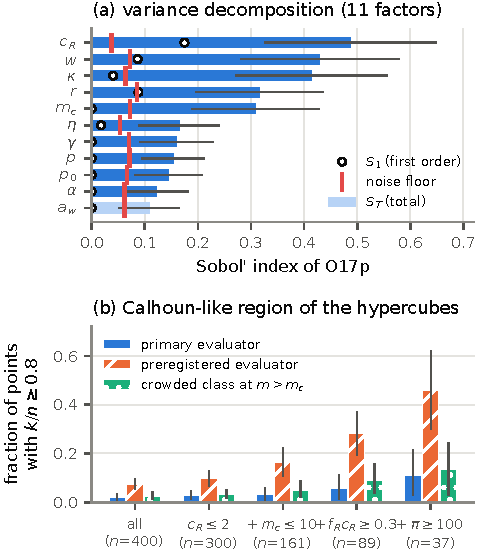
\includegraphics[width=0.55\textwidth]{fig_pre_global.pdf}
  \caption{Global sensitivity around \textsf{C1} (primary evaluator). \textbf{(a)}~Sobol' total indices $S_T$ of
  O17p (bars, bootstrap intervals), first-order indices $S_1$ (open circles) and empirical noise floor (red ticks);
  Saltelli design with $N=256$, 11 factors, 6 runs per point. Dark bars meet the relevance criterion
  $S_T-S_T^{\rm noise}>0.05$ with the lower confidence bound above the floor. \textbf{(b)}~Fraction of Calhoun-like
  points ($k/n\ge0.8$) of the two Latin hypercubes in nested subsets chosen after the runs ($c_R\le2$, then
  $m_c\le10$, $f_Rc_R\ge0.3$ and $\pi\ge100$), with bootstrap intervals, for the primary evaluator, the preregistered
  evaluator and the primary evaluator with the crowded class at $m>m_c$.}
  \label{fig:supp-global}
\end{figure}

\begin{table}[ht]
\centering
\caption{Lattice side $L$ at fixed seeding density $N_0/L^2=0.44$ ($n=60$ per size, $T=600$). Medians over runs;
$t_{\rm last}$ is the last surviving birth, $D_{\rm last}=T_{\rm ext}-t_{\rm last}$; the spread is the interquartile
range over the median of the Kaplan--Meier estimate of $T_{\rm ext}$, with bootstrap interval.}
\label{tab:res-size}
\footnotesize
\setlength{\tabcolsep}{3.5pt}
\begin{tabular}{@{}rrrlcccrrrrl@{}}
\toprule
$L$ & $N_0$ & $n$ & O17p & $\rho_{\rm pk}$ & $f_0$ & $\Phi^{\rm pers}_{\rm BO}$ & $t_{\rm last}$ & IQR & $D_{\rm last}$ & $T_{\rm ext}$ & spread \\
\midrule
15 & 100 & 60 & 0.82 [0.70, 0.89] & 0.35 & 0.18 & 0.18 & 50 & 29 & 110 & 162 & 0.148 [0.121, 0.194] \\
20 & 178 & 60 & 0.90 [0.80, 0.95] & 0.36 & 0.17 & 0.17 & 62 & 22 & 112 & 175 & 0.143 [0.110, 0.169] \\
30 & 400 & 60 & 0.98 [0.91, 1.00] & 0.37 & 0.16 & 0.17 & 58 & 13 & 110 & 170 & 0.076 [0.053, 0.112] \\
45 & 900 & 60 & 1.00 [0.94, 1.00] & 0.37 & 0.15 & 0.17 & 66 & 16 & 111 & 176 & 0.085 [0.052, 0.113] \\
60 & 1600 & 60 & 1.00 [0.94, 1.00] & 0.37 & 0.15 & 0.17 & 75 & 14 & 110 & 184 & 0.076 [0.050, 0.103] \\
\bottomrule

\end{tabular}
\end{table}

\section{Ensembles}
\label{supp:ensembles}

Table~\ref{tab:res-ensembles} lists every ensemble of the production program with its size, horizon and base seed, so that each number of the main text can be traced to its source. Seeds are derived as
\texttt{SeedSequence([base\_seed, point, replicate])}; the base seeds of the production runs (25301--25336) differ
from those of the runs of the preregistered design, so the two sets of runs are independent. The program comprises 51\,828
simulations and 960 transplant replicates in 26 stages, about 4.4 hours of logged wall time on four cores, 1.8 of
them for the Sobol' design; a run of \textsf{C1} or one of its variants costs 0.5--2.6\,s of CPU time.

\begin{table}[ht]
\centering
\caption{Ensembles of the production program (\texttt{results\_v2/f2b\_<stage>} in the code repository). Points:
design points or arms; per point: runs or transplant replicates; $T$: horizon in weeks; seed: base seed of the
stage.}
\label{tab:res-ensembles}
\scriptsize
\setlength{\tabcolsep}{4pt}
\begin{tabular}{@{}llrrrrrl@{}}
\toprule
Stage & Content & points & per point & runs & $T$ & seed & used for \\
\midrule
\texttt{base} & reference ensemble: C1, C1$'$, C0, $\alpha=0$ & 4 & 200 & 800 & 600 & 25301 & production \\
\texttt{c1c2} & C1 and C2 & 2 & 200 & 400 & 700 & 25318 & QC \\
\texttt{ref} & short-lived and long-lived controls & 2 & 100 & 200 & 1000 & 25302 & Q3, controls \\
\texttt{nulos} & four null models & 4 & 200 & 800 & 600 & 25330 & discrimination \\
\texttt{abl1} & single ablations and variants & 9 & 120 & 1080 & 600 & 25303 & Q2 \\
\texttt{abl2} & double to quadruple ablations, $\gamma=0$ & 12 & 40 & 480 & 600 & 25304 & ablations \\
\texttt{trans} & 8 transplant arms, 11 phases & 8 & 60 & 480 & 300 & 25306 & Q1, O12 \\
\texttt{amax} & $a_{\max}\in\{90,\dots,150\}$ & 5 & 60 & 300 & 600 & 25305 & Q4 \\
\texttt{rob} & demographic and update variants & 16 & 200 & 3200 & 700 & 25331 & robustness \\
\texttt{ci} & non-synchronous initial condition & 4 & 200 & 800 & 700 & 25333 & robustness \\
\texttt{size} & $L\in\{15,\dots,60\}$ at fixed density & 5 & 60 & 300 & 600 & 25334 & size \\
\texttt{q7aw} & $a_w$ varied at $\gamma=0$ & 54 & 20 & 1080 & 600 & 25335 & Q7 \\
\texttt{p1} & plane $(r,w)\times\gamma$ & 112 & 30 & 3360 & 600 & 25309 & Q7, P1 \\
\texttt{p1aw} & plane $(r,a_w)$ & 56 & 30 & 1680 & 600 & 25310 & Q6 \\
\texttt{p2} & plane $(\alpha,\kappa)$, $p$ & 72 & 30 & 2160 & 600 & 25308 & Q5, P2 \\
\texttt{p5} & refuge plane & 50 & 30 & 1500 & 600 & 25311 & P5 \\
\texttt{lhs} & Latin hypercube 1 & 200 & 10 & 2000 & 400 & 25312 & global \\
\texttt{lhs2} & Latin hypercube 2 & 200 & 10 & 2000 & 400 & 25313 & global \\
\texttt{lhsx} & boundary points of the hypercubes & 18 & 40 & 720 & 400 & 25336 & global \\
\texttt{morris} & Morris screening & 320 & 10 & 3200 & 400 & 25307 & global \\
\texttt{sobol} & Saltelli design, 11 factors & 3328 & 6 & 19968 & 400 & 25314 & global \\
\texttt{robmu} & $\mu_{\rm bg}$ curve & 12 & 60 & 720 & 700 & 25332 & robustness \\
\texttt{p4} & seeding density and lattice & 24 & 30 & 720 & 600 & 25315 & P4 \\
\texttt{trgrid} & transplants on $(\alpha,\kappa)$ & 12 & 40 & 480 & 300 & 25316 & O12 \\
\texttt{refine} & 40 boundary points of the planes & 40 & 100 & 4000 & 600 & 25317 & planes \\
\texttt{p6} & founder protocol & 12 & 30 & 360 & 900 & 25319 & O1--O3 \\
\bottomrule

\end{tabular}
\end{table}

\section{Deviations from the preregistration}
\label{supp:deviations}

Table~\ref{tab:deviations} lists every deviation from the preregistered plan (\texttt{docs/preregistered\_plan.md} in the
code repository, dated 1 October 2026, 22:02 UTC, before the launch of the production runs), including the
redefinition of the primary evaluator, and the analyses labelled post hoc.

\begin{table}[ht]
\centering
\caption{Deviations from the preregistered plan and post hoc analyses. ``Before production'' means after the
calibration but before the production runs; ``post hoc'' means after the runs had been seen. The last block lists
the changes that are not preregistered but were fixed, with their decision rules, before the production runs
(\texttt{docs/production\_plan.md} in the code repository, 2 October 2026, 05:34 UTC).}
\label{tab:deviations}
\scriptsize
\setlength{\tabcolsep}{3pt}
\begin{tabular}{@{}p{5.2cm}p{2.8cm}p{4.4cm}p{4.0cm}@{}}
\toprule
Change & When & Affects & Treatment \\
\midrule
O13p (persistent isolated class) defined and made part of the primary outcome, together with R7 & before
production, after seeing that \textsf{C0} has no persistent class & O17p, Q2, necessity of R7 & declared as
circular for R7 (main text, Discussion) \\
O6: rebound count also detects slow regrowth still rising at censoring & post hoc (2 Oct., 02:44) & one
\textsf{C1} run of 200 under the preregistered design; none in the production runs & primary evaluator \\
O13b: reading of the window against the median birth week & post hoc & the interpretation of O13b in \textsf{C1}
and \textsf{C2} & labelled post hoc \\
Robust spread of $T_{\rm ext}$ (Kaplan--Meier interquartile range over median) & post hoc (the plan had
$\mathrm{CV}\le0.10$ for Q3) & the claims about the spread of the extinction time & labelled post hoc; the
equivalence of \textsf{C1}$'$ with the long-lived control found under the preregistered design does not hold in the production runs \\
Ensembles of \textsf{C1}$'$ and the \textsf{C1}--\textsf{C1}$'$ contrast & post hoc & minimality, the role of AV &
labelled post hoc \\
Subsets of the hypercubes (nested conditions on $c_R$, $m_c$, $f_Rc_R$, $\pi$) & post hoc & interpretation of the
Calhoun-like fraction & descriptive only \\
Re-scoring with other class thresholds $\theta$ and ensemble thresholds $\tau$ (Sec.~\ref{supp:null}) & post hoc & conditionality of minimality & descriptive only \\
Cure model for the extinction time & post hoc & survival summaries & no test reported \\
Holm $p$-value of Q6 computed from the binomial likelihood & as planned & Q6 & the quasi-binomial value enters the
Holm sequence; no decision changes \\
\midrule
\multicolumn{4}{@{}l}{\emph{Not preregistered, fixed before the production runs}}\\
Hard refuge capacity enforced strictly (pups and rejected movers counted); the single-pass admission kept as a variant &
before the production runs & every stage with refuges; all stages run with seeds different from those of the preregistered design & both admission rules reported side by side
(no change in O17p) \\
Primary evaluator redefined: peak time at the start of the plateau ($t'_{\rm pk}$); end of natality in O5 at 99\%
of the births; O4 also requires free space at the peak ($f_0\ge0.10$, an informal target of the calibration);
crowded class $m>8$, independent of $m_c$; O10 on the adult social state; O11 on the second half of the births, not
applicable when the late cohorts are empty; NA counts as failure in O17p & fixed after exploratory runs with the primary evaluator and before the production runs & every pattern
normalised by $t_{\rm pk}$, O4, O5, O10, O11, O13, O13p, O17p in every stage; the verdicts of Q1 (prediction), Q2
(null) and Q6 (prediction) & the full preregistered evaluator, and each option changed separately, reported next to the
primary one (Table~\ref{tab:res-rescoring}) \\
O5 birth reference $t_{B99}$ instead of the last sustained birth $t_{\rm last}$ & after exploratory runs had
shown that $t_{\rm last}$ with $t'_{\rm pk}$ fails O5 in most \textsf{C1} runs (0.48 in the production runs,
Table~\ref{tab:res-rescoring}); a choice informed by the result & Q2: it is the only option on which the rejection
of its null hypothesis depends (with the preregistered evaluator 5 of 7 null hypotheses are rejected and Q2 is not;
with the primary one, 6 of 7) & both birth references reported for every arm; the count with the preregistered
evaluator given next to the primary one \\
Confirmatory test of the equivalence of the exponents of $r$ and $a_w$ at $\gamma=0$ (TOST, margin $[2/3,3/2]$,
stage $a_w$ varied) & before the production runs & Q7 with $a_w$ varied & the design cannot carry it out as inference
(51 of 54 points at $P_{\rm ext}\in\{0,1\}$, separated logistic); replaced by a non-parametric summary per window
(Sec.~\ref{supp:Q}); the planned estimates are kept, labelled, in \texttt{results\_numbers.json} \\
O8 (senescent decline) of \textsf{C1}: 0.71 under the preregistered design, 0.62 in the production runs (0.64 with the
single-pass admission and the seeds of the production runs) & observed after the production runs & a desirable pattern; no
decision & reported; not a conclusion \\
Transplant of Q1 taken at $1.75\,t'_{\rm pk}$ instead of $1.75\,t_{\rm pk}$; sampling at a common week added &
before the production runs & Q1, O12 & both times reported; comparisons between arms only at equal time \\
Sobol' design with 11 factors (the 8 selected by Morris plus $w$, $r$, $a_w$) & before the production runs & global
sensitivity & indices conditional on the 4 fixed factors \\
Additional stages: null models, demographic and update variants, non-synchronous initial condition, transplants of
intermediate animals, extra replicates at the hypercube boundary, $a_w$ varied at $\gamma=0$ (additional confirmatory test), lattice size & before the production runs & robustness, discrimination, Q1, Q7, feasible region & decision rules fixed before the runs \\
\bottomrule
\end{tabular}
\end{table}

\section{Condensed model description (ODD protocol)}
\label{supp:odd}

We follow the second update of the ODD protocol \cite{Grimm2020}; the full description is in \extended.
Parameter names refer to the \texttt{Params} class of the \texttt{u25} package.

\paragraph{Purpose and patterns.}
The purpose is to identify a minimal set of \emph{local} rules that, with unlimited resources and without
thresholds on the total population, generates the qualitative sequence reported for Universe~25: latency,
exponential growth, deceleration with social deterioration, cessation of surviving births near the peak, decline
without recovery to extinction, and differentiated classes of deteriorated animals. The model is evaluated against
the patterns of Table~\ref{tab:observations-full} and, for each pattern, against null models. With the default
initial condition only items 3--6 are testable, and the model reproduces them as a boom of one or two generations
followed by extinction by senescence; of these items, the crowding damage and the demography already give the end
of natality and the decline, and the rules add the classes.

\paragraph{Entities, state variables and scales.}
Each agent carries an identifier, a sex $\sigma_i\in\{M,F\}$ fixed at birth, a cell $(x_i,y_i)$ on an $L\times L$
lattice with hard walls ($L=30$), an age $a_i$ in weeks, a social state $s_i\in[0,1]$ ($1$ = full social competence)
and, in \textsf{C2}, the maternal social state at birth $h_i$. Each pair carries a symmetric affinity
$F_{ij}\in[0,1]$, stored sparsely (pairs with $F_{ij}<\varepsilon$ are pruned). Ordinary cells have no occupancy
limit; a fixed random fraction $f_R$ of cells are \emph{refuges} with capacity $c_R$, drawn once
(\texttt{refuge\_seed}${}=0$) and identical in every run (eight alternative layouts gave no
detectable difference). One time step is one week. A cell is an abstract meeting place, mapped to a nest box of
Universe~25, the damage threshold $m_c$ to its comfortable occupancy and $K_\gamma=L^2m_c=7200$, the population at
which every cell would sit at the damage threshold, to Calhoun's 3840 places; $K_\gamma$ is a reference for the peak
density, not a physical capacity, and $|G|$ and $m_c$ were not calibrated. The refuges correspond to the
little-preferred high nests; their capacity $c_R=2$ is the isolation threshold of O13, not the capacity of a nest.
Mobility is at most one Moore step per week, so the ratio of the mixing time to the deterioration time (a
Damk\"ohler number) is about $1.7\times10^2$ in \textsf{C1}, against $\lesssim4\times10^{-3}$ in Universe~25.

\paragraph{Process overview and scheduling.}
Each week, in order: (1) movement, simultaneous, with weights evaluated on the pre-move snapshot, with refuge
capacity enforced after the move (an asynchronous variant, agents moving one at a time in random order, is a
robustness check); (2) affinity update; (3) occupancy $m_i$ after movement, including $i$ itself; (4) social-state
update; (5) reproduction; (6) ageing; (7) mortality; (8) recording of observables. Updates within each submodel are
synchronous.

\paragraph{Design concepts.}
\emph{Basic principles:} social stress from crowding reduces reproduction and offspring survival
\cite{Christian1950,Southwick1955}; maternal transmission of individual quality
\cite{GinzburgTaneyhill1994,InchaustiGinzburg1998}; the behavioural sink, attraction to familiar individuals
producing aggregation despite free space \cite{Calhoun1962,Calhoun1973}. \emph{Emergence:} the population
trajectory, the spatial aggregation, the effective deterioration threshold and the classes of crowded and isolated
deteriorated animals are not imposed by any rule; imposed by design, and therefore consistency checks, are the
irreversibility of adults (R1) and with it the failure of transplanted late-phase animals, the persistence of the
isolated class in refuges of capacity $c_R=2$, and the absence of social deaths and the senescent decline, since
social mortality is off. \emph{Adaptation, objectives, learning, prediction:} agents do not optimize anything;
``social learning'' (R2) is a contagion rule. \emph{Sensing:} agents sense only their Moore neighbourhood (their
affinities with the occupants of each neighbouring cell, the occupancy of those cells, the mean social state of
neighbours, and whether a cell is a refuge and is full); no rule uses the total population size.
\emph{Interaction:} co-presence (affinity), mating within the cell, social learning and crowding.
\emph{Stochasticity:} destination choice; mate choice, conception, litter size, neonatal survival and sex; death;
the order of entry into full refuges and the relocation cell when a refuge is full; in the asynchronous variant the
order of moves; in the non-synchronous variant the initial ages. The state $N=0$ is absorbing.
\emph{Observation:} per-step time series, per-run summaries and the automatic pattern evaluator.

\paragraph{Initialization and input.}
Default: 200 males and 200 females aged 4 weeks with $s=1$, placed uniformly at random, with no affinities (a
synchronous cohort; integer ages drawn uniformly between 4 and 52 or between 4 and 80 weeks are a robustness
check). Founders: 4 males and 4 females aged 7 weeks with $s=1$ in the central cell. Transplant: 4 males and 4
females of reproductive age taken from a donor run, keeping their $s$, placed in the central cell of an empty
lattice. There is no input data: no resource limitation, predation or emigration.

\paragraph{Submodels.}
\emph{Movement.} Agent $i$ chooses a destination $y$ in its Moore neighbourhood $V(i)$, which includes its own
cell, with weight
\[
w_i(y)=\bigl[1+\alpha A_i(y)\bigr]\,e^{-\kappa(1-s_i)^{p}n_y}\,
\bigl[1+\pi\,(1-b_i)^{q}\,\mathbf 1_{\mathcal R}(y)\bigr],\qquad
A_i(y)=\sum_{j\in y,\,j\ne i}F_{ij},
\]
where $n_y$ is the occupancy of $y$ excluding $i$, $\mathbf 1_{\mathcal R}(y)=1$ if $y$ is a non-full refuge
($n_y<c_R$) and 0 otherwise, $\kappa$ and $p$ define the aversion of the deteriorated (AV),
$\pi$ and $q$ the refuge preference (R7), and $b_i=s_i$ in \textsf{C1} and $b_i=h_i$ in \textsf{C2}. Full refuges
cannot be entered: residents have priority, entering agents are drawn in random order, rejected agents return to
their previous cell, and admission is iterated to a fixed point (\texttt{refuge\_hard="strict"}); pups, founders
and transplanted animals that would put a refuge above capacity are placed in a uniformly chosen non-refuge cell
of the nearest Chebyshev ring that contains one. A single-pass admission, which does not count returning agents and newborns, is kept as a robustness variant.
\emph{Affinity.} If $i$ and $j$ are at Chebyshev distance $\le1$ after movement, $F_{ij}\leftarrow(1-\eta)F_{ij}+\eta$;
otherwise $F_{ij}\leftarrow(1-\delta)F_{ij}$.
\emph{Social state.}
\[
s_i\leftarrow\Pi_{[0,1]}\Bigl(s_i+r\,\mathbf 1_{a_i\le a_w}\bigl[(1-\lambda)+\lambda\,\bar s_{V(i)}\bigr]
-\gamma\,(m_i-m_c)_+\Bigr),
\]
where $r$ is the recovery (learning) rate, $\bar s_{V(i)}$ the mean social state of the \emph{other} agents in
$V(i)$ (zero if there are none), $a_w$ the plasticity window (R1) and $\lambda$ the social-learning weight (R2); the
neutral values $a_w=\infty$ and $\lambda=0$ (with $w=1$ and $r=0.01$) recover the core model.
\emph{Reproduction.} Each reproductive female ($a_{\min}\le a\le a_{\rm rep}$) that shares her cell with at least
one reproductive male chooses one uniformly at random and conceives with probability $p_0s_fs_m$; the litter size
is drawn from an empirical distribution on $\{3,\dots,10\}$ (mean $6.55$) and Binomial$(L,q_0s_f)$ pups survive,
with $q_0=0.95$. Pups are born in the mother's cell at age 0, with sex ratio $1/2$ and social state
$s=w\,s_f+(1-w)\,s_{\rm base}$ (with $w=0.2$ and $s_{\rm base}=0$ every pup is born with $s\le0.2$); they are
independent agents from birth and add to local crowding (a nest period of three weeks is a robustness check).
\emph{Mortality.} After ageing, each agent dies with probability $1/(1+e^{-k(a-a_{\max})})$. Social mortality is
switched off in all presets; a background hazard $\mu_{\rm bg}$ at all ages, combined as
$1-(1-p_{\rm age})(1-\mu_{\rm bg})$, is a robustness check.

\begin{table}[ht]
\centering\small
\caption{Parameters of the short-lived control (SL), values in \textsf{C1}, and justification. [E] empirical, [O]
order of magnitude, [M] modelling choice, [C] calibrated qualitatively. \textsf{C1}$'$ is \textsf{C1} with
$\kappa=0$; \textsf{C0} is \textsf{C1} without refuges; \textsf{C2} has $\pi=1000$, $q=1$ and the maternal basis
$b_i=h_i$.}
\label{tab:odd-params}
\begin{tabular}{@{}p{0.26\textwidth}p{0.10\textwidth}p{0.12\textwidth}p{0.44\textwidth}@{}}
\toprule
Parameter & SL & \textsf{C1} & Justification \\
\midrule
\texttt{grid\_size} $L$ & 30 & 30 & [M] abstract space; Calhoun had 16 cells, 256 nest boxes \\
$N_0$ & 200+200 & 200+200 & [M]; founders 4+4 as in \cite{Calhoun1973} \\
\texttt{initial\_age} & 4 & 4 & [M]; 7 for founders (48 days) \\
$\eta$, $\delta$, $\varepsilon$ & 0.2, 0.01, $10^{-6}$ & same & [M] bond formation $\sim$5 weeks, memory $\sim$100 weeks \\
$\alpha$ & 1.4 & 4 & [C] attraction to familiar individuals (behavioural sink) \\
$m_c$ & 8 & 8 & [M/O] ``Fifteen mice could comfortably rest in a single nest box''; groups of ``over 10 individuals'' \cite{Calhoun1973} \\
$r$ (\texttt{rec}) & 0.01 & 0.1 & [M/C] recovery/learning rate \\
$\gamma$ & 0.1 & 0.1 & [M] damage per excess occupant \\
$p_0$ & 0.3 & 0.3 & [O] weekly conception probability given an encounter \\
$q_0$ & 0.95 & 0.95 & [M] \\
$a_{\min}$ & 6 & 6 & [O] sexual maturity $\approx$6 weeks \\
$a_{\rm rep}$ & 50 & 80 & [E] menopause at ``about 560 days'' $\approx$80 weeks \cite{Calhoun1973} \\
litter sizes & 3--10, mean 6.55 & same & [O] mean 6.12 in the source of \cite{GwizdallaDus2026} \\
$a_{\max}$, $k$ & 60, 0.15 & 120, 0.15 & [E] ``large numbers'' lived to 800 days; last survivors $>987$ days \cite{Calhoun1973} \\
$a_w$ (R1) & $\infty$ & 12 & [C] juvenile plasticity window \\
$\lambda$ (R2) & 0 & 1 & [C] social learning \\
$w$, $s_{\rm base}$ & 1, 1 & 0.2, 0 & [C] partial maternal inheritance \\
$\kappa$, $p$ (AV) & 0, 1 & 0.15, 4 & [C] crowd aversion of deteriorated animals \\
refuge fraction, capacity & 0, -- & 0.3, 2 (hard) & [C] R7; layout \texttt{refuge\_seed}${}=0$ \\
$\pi$, $q$, basis (R7) & 0 & 100, 4, current & [C]; \textsf{C2}: 1000, 1, maternal \\
\texttt{max\_pop} & 60000 & 15000 & numerical safeguard \\
\bottomrule
\end{tabular}
\end{table}

\section{Further details of the model}
\label{supp:model}
\InputIfFileExists{sections/supp_model}{}{%
The complementary material of the model section (the dimensionless groups, the scales and the generation
register) is given in \extended.}

\bibliographystyle{apsrev4-2}
\bibliography{refs}

\end{document}
